\section{Conclusions}
    \begin{frame}
    \frametitle{Outline}
    \begin{columns}[T]
        \begin{column}{.45\textwidth}
            \tableofcontents[sections=1-3,currentsection]
        \end{column}
        \begin{column}{.45\textwidth}
            \tableofcontents[sections=4-5,currentsection]
        \end{column}
    \end{columns}
    \end{frame}


\subsection{Configurations Comparison}
\begin{frame}{\subsecname}

\begin{minipage}[t]{0.5\linewidth}
\begin{figure}[H]
    \centering
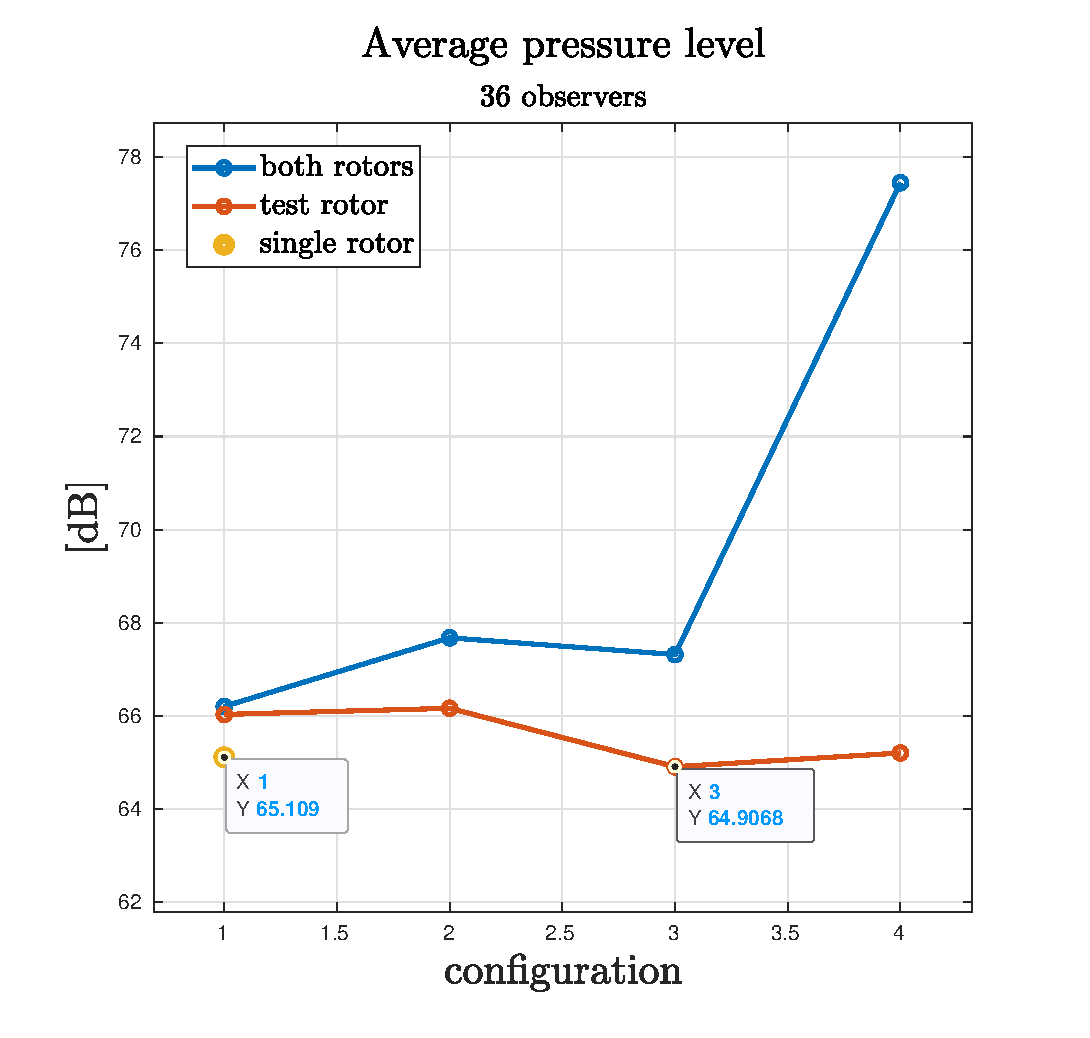
\includegraphics[scale=0.36]{Photos/averageSPL_config_comparison.eps}
\end{figure}  
\end{minipage}\hfill
\begin{minipage}[t]{0.43\linewidth}
\vspace{2cm}
\resizebox{5cm}{!}{
 \begin{table}[H]
                %\caption*{\textbf{Title of Table (optional)}}
                \centering 
                \begin{tabular}{|c c c|}
                \hline
                \rowcolor{bluePoli!40 } % bluePoli!40 comment this line to remove the color
                Config & 1 rotor [dB] & 2 rotors [dB] \T\B \\
                \hline \hline
                1 (040.000) & 66.03  & 66.20 \T\B  \\
                2 (031.000) & 66.16 & 67.68 \T\B  \\
                3 (030.010) & 64.91 & 67.32 \T\B  \\
                4 (025.010) & 65.20 & 77.45 \T\B  \\
                \hline \hline
                Single Rotor & 65.11 & \T\B  \\
                \hline
                \end{tabular}
    \end{table} }
    
\end{minipage}





\end{frame}


\begin{frame}
   \begin{itemize}
       \item Sound gets \textbf{reduced} with:
       \begin{itemize}
        \item Increasing rotor axis distance
        \item Adding a stagger
       \end{itemize}

       \item Sound gets \textbf{amplified} when Blade Vortex Interaction occurs

       \item \textbf{Aerodynamic performance}:
       \begin{itemize}
           \item Similar behavior for non-wake interference configurations
           \item The more the wake interaction, the more reduction in performance
       \end{itemize}

       \item \textbf{Tonal Noise} is attributed to the Blade Passing Frequency

       
   \end{itemize}
\end{frame}

 \subsection{Further Investigation}
 \begin{frame} {\subsecname}
     \begin{itemize}
         \item Observers located in the vertical plane
         \item Changing the stagger distance $\xrightarrow{}$ Find the optimal configuration
         \item Validation with numerical or experimental data
         \item Aeroacoustic study of the nacelles' influence
     \end{itemize}
 \end{frame}

\subsection{Preliminary nacelle results}

\begin{frame} {\subsecname}
    \begin{figure}
\centering
\begin{minipage}{.5\textwidth}
  \centering
  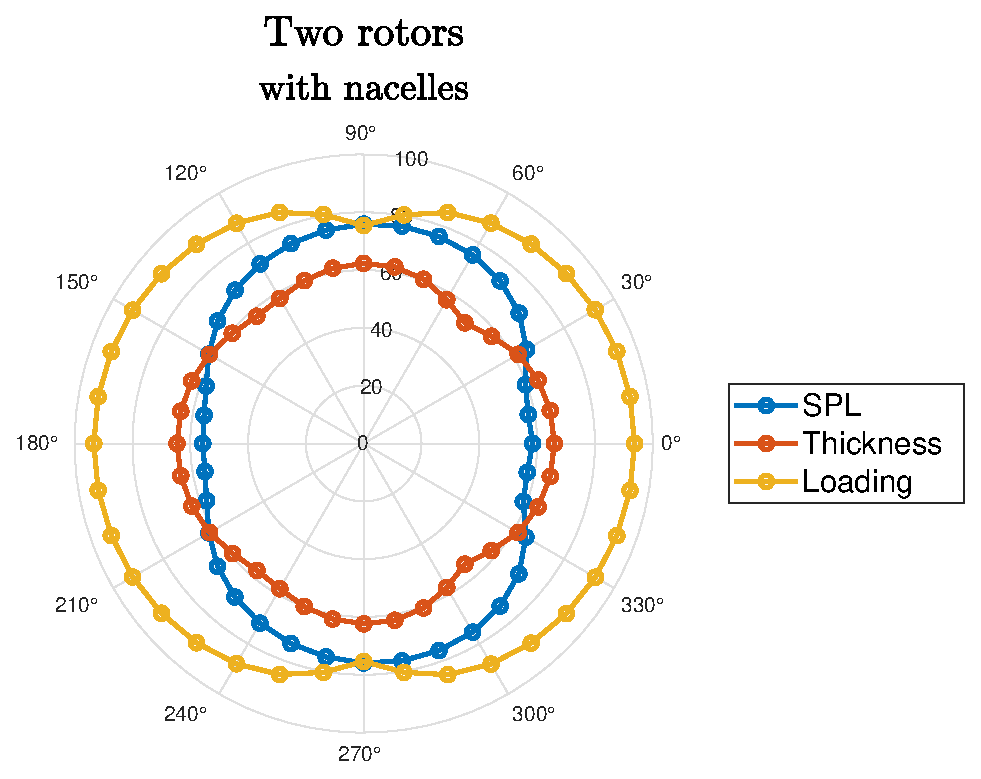
\includegraphics[scale=0.35]{Photos/spl_thick_load_nacelles.eps}
\end{minipage}%
\begin{minipage}{.5\textwidth}
  \centering
  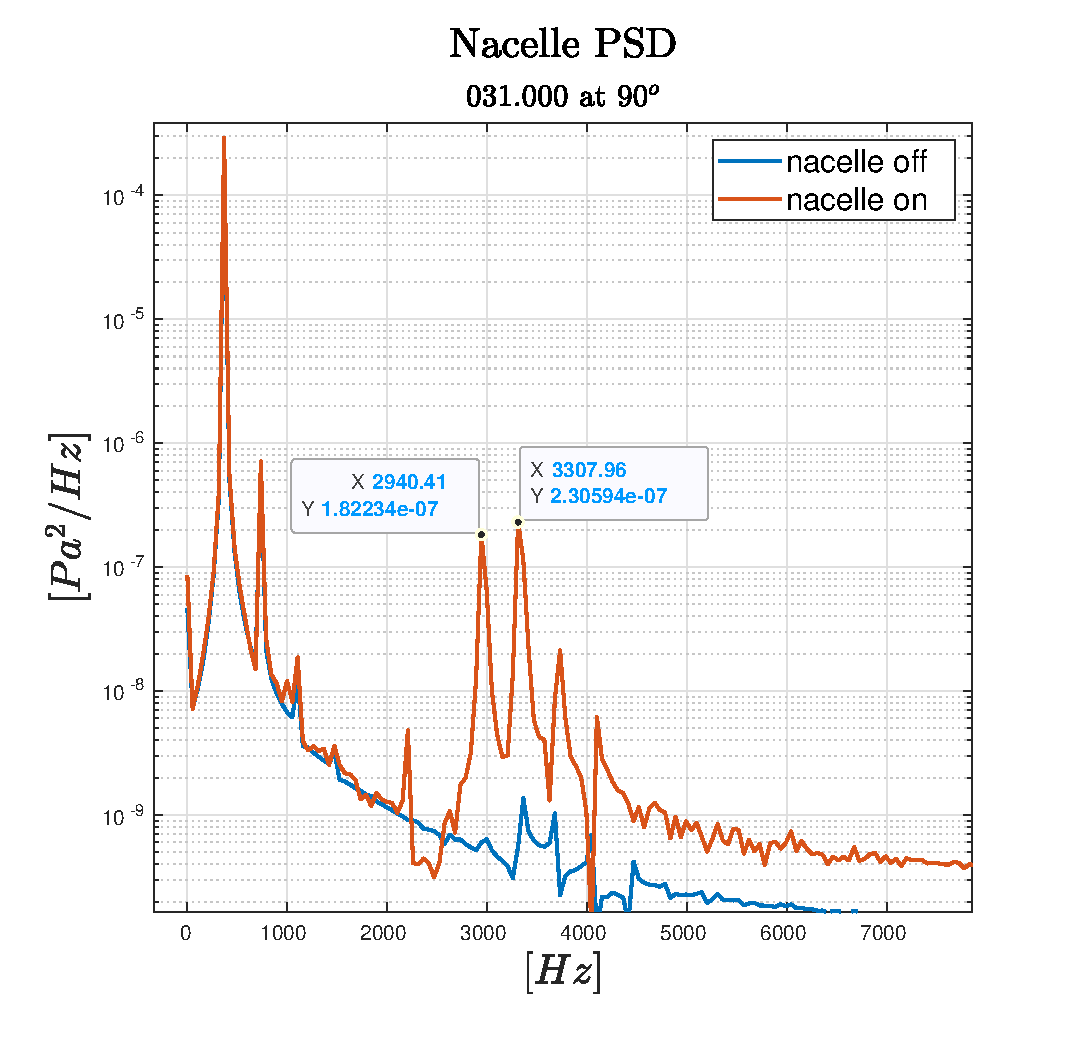
\includegraphics[scale=0.35]{Photos/psd_nacelle.eps}
\end{minipage}
\end{figure}
\end{frame}